\chapter{Cifras de Fluxo}
\label{cha:cifras-de-fluxo}

No capítulo anterior, apresentamos uma definição formal para segurança contra ataques em que o adversário tem acesso apenas ao texto cifrado.
Neste capítulo, vamos apresentar uma forma de construir um sistema que satisfaz essa definição.

A ideia geral da construção é a seguinte:
partimos de uma sequência aleatória de bits chamada de semente e, a partir dela, geramos uma sequência maior de bits para encriptar a mensagem usando a operação de OU exclusivo (XOR), assim como no OTP.
Embora essa sequência seja gerada de maneira determinística, a segurança do sistema depende do fato de que ela se pareça aleatória.

Informalmente, um {\em Gerador de Números Pseudoaleatórios} (GNP) é uma função que recebe uma semente aleatória e a expande em uma sequência maior que aparenta ser aleatória.
A qualidade de um GNP é medida pela sua capacidade de produzir sequências que são indistinguíveis de sequências verdadeiramente aleatórias para qualquer adversário eficiente.

Sistemas de cifra de fluxo foram estudados extensamente nos anos 80 \cite{Blum84,Yao82}.
A abordagem para verificar se o gerador de números pseudoaleatórios é suficientemente forte consistia em aplicar uma série de testes estatísticos na sequência gerada para tentar distingui-la de uma sequência aleatória.

Por exemplo, um teste pode verificar se a probabilidade de o primeiro bit da sequência ser igual a $1$ é $1/2$.
Isso significa que, em uma sequência verdadeiramente aleatória, a chance de o primeiro bit ser $1$ deve ser igual à chance de ser $0$, ou seja, $50\%$.
O teste verifica se essa propriedade é mantida na sequência gerada pelo GNP.
Se a sequência gerada tiver uma probabilidade significativamente diferente de $1/2$ para o primeiro bit ser $1$, isso pode indicar que a sequência não é suficientemente aleatória.

Outro exemplo de teste é verificar se a probabilidade de ocorrência de pelo menos três $0$s em qualquer subsequência de tamanho 4 é $5/16$.
Para entender por que essa é a probabilidade esperada, consideremos todas as possíveis subsequências de 4 bits:

\begin{itemize}
\item Existem exatamente 1 subsequência onde todos os bits são $0$s ($0000$).
\item Existem 4 subsequências onde três dos quatro bits são $0$s ($0001$, $0010$, $0100$, $1000$).
\end{itemize}

Portanto, há 5 subsequências que atendem ao critério (1 com quatro $0$s e 4 com três $0$s) em um total de $2^4 = 16$ possíveis subsequências de 4 bits.
Assim, a probabilidade de ocorrência de pelo menos três $0$s em uma subsequência de 4 bits é $5/16$.

O teste então verifica se a sequência gerada pelo GNP possui essa distribuição específica de $0$s em suas subsequências de 4 bits.
Se a sequência gerada pelo GNP passar neste teste, isso sugere que a sequência é indistinguível de uma sequência verdadeiramente aleatória em relação a essa propriedade específica.

Devido ao seu papel em diferenciar sequências pseudoaleatórias de sequências verdadeiramente aleatórias, esses testes são chamados de {\em distinguidores}.
Os distinguidores são essenciais para avaliar a robustez de um GNP, pois nos ajudam a garantir que as sequências geradas são adequadamente aleatórias para serem usadas em sistemas de criptografia seguros.

Uma bateria de distinguidores pode ser usada para verificar a qualidade de um GNP.
Idealmente, nenhum teste eficiente deveria ser capaz de distinguir a sequência gerada por um GNP de uma sequência verdadeiramente aleatória, ou pelo menos, deveria ser incapaz de fazê-lo com uma probabilidade considerável\footnote{Usaremos o termo ``considerável'' para probabilidades não desprezíveis.}.

Definimos um Gerador de Números Pseudo-aleatórios (GNP) como um algoritmo $G$ que recebe uma semente $s$ de um determinado tamanho $n$ e produz uma sequência maior de bits de tamanho $l(n)$.
O fator de expansão do GNP, representado pela função $l$, indica quanto maior é a sequência produzida em comparação com a semente inicial.

Para que um GNP seja considerado seguro, a sequência gerada a partir da semente deve ser indistinguível de uma sequência verdadeiramente aleatória.
Em outras palavras, não deve ser possível para nenhum algoritmo eficiente distinguir entre a sequência gerada pelo GNP e uma sequência aleatória com uma probabilidade significativa.

Em outras palavras, um GNP é seguro se para todo algoritmo polinomial $D$ (distinguidor), a diferença na probabilidade de $D$ identificar corretamente a origem da sequência ($|Pr[D(r) = 1] - Pr[D(G(s)) = 1]|$) for desprezível.

A restrição de que o distinguidor seja eficiente é estritamente necessária.
Isso se deve ao fato de que, em teoria, sempre é possível construir um distinguidor usando uma espécie de ataque de força bruta.
Vamos explorar como isso funciona.

Imagine que temos uma sequência de bits $w$ e queremos saber se ela foi gerada por um GNP $G$  se é uma sequência verdadeiramente aleatória.
Um algoritmo $D$, nosso distinguidor, pode realizar a seguinte estratégia:

\begin{enumerate}
    \item Para cada possível semente $s$, o algoritmo $D$ verifica se $G(s) = w$  . 
    \item Se encontrar uma semente $s$ tal que $G(s) = w$, $D$ devolve $1$ (indicando que a sequência foi gerada pelo GNP).
    \item Se não encontrar nenhuma semente que gere $w$, $D$ devolve $0$ (indicando que a sequência é aleatória).
\end{enumerate}

Para uma semente de $n$ bits, existem $2^n$ possíveis combinações.
Como apenas uma dessas combinações de $s$ gera $w$ corretamente, a chance de $D$ encontrar essa combinação é $\frac{1}{2^n}$.

Além disso, esse teste é que ele não é eficiente.
Para testar todas as possíveis sementes $s$, o tempo esperado é exponencial, mais precisamente $2^{n-1}$.
Esse tempo de execução torna o método impraticável para valores grandes de $n$.
Portanto, embora seja teoricamente possível distinguir sequências geradas por um GNP de sequências aleatórias usando força bruta, na prática, a restrição de que o distinguidor seja eficiente é essencial para garantir que o GNP seja útil e seguro.

\section{Segurança das Cifras de Fluxo}
\label{sec:streamcipher-sec}

Como adiantamos no capítulo anterior, uma vez definida claramente a suposição que estamos fazendo, podemos tentar provar que, com essa suposição, somos capazes de construir um sistema seguro.
A abordagem para este tipo de prova é uma redução, similar às reduções que vimos em Teoria da Computação.
Neste caso, vamos reduzir o problema de construir um sistema seguro contra ataques contra o texto cifrado apenas ({\em ciphertext-only}) ao problema de construir um GNP.

Reduções são ferramentas poderosas em teoria da computação e criptografia.
Elas nos permitem transformar um problema desconhecido ou difícil em um problema conhecido ou mais simples.
Se conseguirmos mostrar que resolver um problema implica resolver outro problema, estabelecemos uma relação de dependência entre eles.
Neste contexto, se pudermos construir um GNP seguro, podemos utilizar esse GNP para construir um sistema de criptografia que seja seguro contra ataques ciphertext-only.

O processo de redução pode ser descrito da seguinte maneira:

\begin{itemize}
\item[] {\em Definir a Suposição}:
  Primeiro, definimos claramente a suposição que estamos fazendo, no caso, a existência de um GNP seguro.
  Um GNP seguro é um gerador que produz sequências de bits que não podem ser distinguidas de sequências verdadeiramente aleatórias por qualquer algoritmo eficiente.

\item[] {\em Transformar o Problema}:
  Em seguida, transformamos o problema de construir um sistema seguro contra ataques ciphertext-only em um problema que envolve o GNP.
  Mostramos que, se temos um GNP seguro, podemos usar esse GNP como base para criar um sistema de criptografia que resista a ataques ciphertext-only.

\item[] {\em Prova de Segurança}:
  Finalmente, provamos que o sistema de criptografia resultante é seguro sob a suposição de que o GNP é seguro.
  Isso geralmente envolve demonstrar que qualquer ataque bem-sucedido ao sistema de criptografia implicaria em um ataque bem-sucedido ao GNP, o que contradiria a suposição de que o GNP é seguro.
\end{itemize}

Essa abordagem de redução nos permite construir sistemas de criptografia confiáveis baseando-nos em componentes cuja segurança já foi estabelecida ou assumida.
Ela também facilita a compreensão das relações entre diferentes problemas de segurança e a reutilização de soluções existentes para resolver novos problemas.

Ao estabelecer essa conexão entre GNPs e sistemas de criptografia, criamos uma base sólida para desenvolver e analisar algoritmos de criptografia modernos, garantindo que nossas construções sejam robustas e confiáveis sob as suposições corretas.

A {\em cifra de fluxo} é um método de criptografia que converte texto claro $m$ em texto cifrado $c$, utilizando um fluxo de chaves pseudoaleatórias gerado por um gerador de números pseudoaleatórios (GNP).
Este método é amplamente utilizado devido à sua eficiência e capacidade de operar em dados de tamanho variável, tornando-o ideal para aplicações como comunicação em tempo real e transmissão de dados.

O processo para criptografar uma mensagem $m$ usando uma cifra de fluxo é o seguinte:
\begin{itemize}
\item Primeiro, uma semente aleatória $k$ de tamanho fixo $n$ é gerada.
  Esta semente deve ser segura e conhecida apenas pelas partes autorizadas.
  Ela será a chave do sistema.
\item A semente é fornecida ao GNP $G$, que expande a semente em um fluxo de chaves $G(k)$ de comprimento adequado para criptografar a mensagem inteira.
\item A mensagem original (texto claro) é combinada bit a bit (ou byte a byte) com o fluxo de chaves usando a operação XOR.
  O resultado é o texto cifrado.

  \begin{displaymath}
    c = m \oplus G(k)
  \end{displaymath}
\end{itemize}

Para descriptografar o processo é similar:
\begin{itemize}
\item A mesma semente $k$ utilizada para criptografar a mensagem é novamente fornecida ao GNP $G$ para gerar o mesmo fluxo de chaves $G(k)$.
\item O texto cifrado é combinado bit a bit (ou byte a byte) com o fluxo de chaves usando a operação XOR.
  \begin{displaymath}
    c \oplus G(k)
  \end{displaymath}
  O resultado é a mensagem original.
\end{itemize}

\begin{theorem}
  \label{theo:stream}
  Uma cifra de fluxo para uma mensagem de tamanho fixo $n$ que utiliza um gerador de número pseudoaleatório para expandir a chave é seguro contra ataques {\em ciphertext only}.
\end{theorem}
\begin{proof}
Para provar o teorema vamos mostrar que se existisse um adversário capaz de quebrar nosso sistema de criptografia, poderíamos usar esse adversário para criar um teste eficiente (distinguidor) que diferencie entre uma sequência gerada por um GNP e uma sequência aleatória.

Vamos supor que temos um adversário que pode quebrar nosso sistema de criptografia.
Isso significa que, dado um texto cifrado, essa adversário consegue determinar informações sobre a mensagem original com uma precisão melhor do que a pura sorte.

Usamos o adversário para construir um distinguidor $D$.
Este distinguidor funciona da seguinte forma:

\begin{enumerate}
  \item $D$ recebe uma sequência $w$ e precisa determinar se $w$ foi gerada por um GNP ou se é uma sequência verdadeiramente aleatória.
  \item $D$ roda o mesmo algoritmo do adversário para obter duas mensagens $m_0$ e $m_1$.
  \item $D$ escolhe aleatoriamente uma das duas mensagens $m$ e calcula $c = w \oplus m$.
  \item $D$ entrega $c$ ao adversário e devolve 1 se ele adivinhar corretamente qual das mensagens foi cifrada e 0 caso contrário.
\end{enumerate}

O distinguidor $D$ que acabamos de construit devolve 1 com a mesma probabilidade com que o adversário consegue quebrar o sistema.
Se $w$ é uma sequência verdadeiramente aleatória, o adversário não terá qualquer vantagem e só poderá adivinhar corretamente com uma probabilidade de $50\%$.

Se o adversário pode quebrar o sistema de criptografia, o distinguidor $D$ pode usar essa capacidade para diferenciar entre uma sequência gerada por um GNP e uma sequência verdadeiramente aleatória.
Isso mostraria que o GNP não é seguro, pois podemos construir um distinguidor eficiente que o quebra.

Ou seja, se o GNP é seguro, então não existe adversário eficiente capaz de derrotar o sistema.
\end{proof}

\begin{center}
  \begin{tikzpicture}

    % Conjunto pequeno
    \node (small) at (0,0) {};

    % Conjunto grande
    \node (large) at (8,0) {};

    % Caixa ao redor do elemento do conjunto pequeno (menor caixa)
    \draw[dashed] ($(small.north west) + (-0.5,0.5)$) rectangle ($(small.south east) + (0.5,-0.5)$);
    
    % Caixa ao redor do elemento do conjunto grande (maior caixa)
    \draw[dashed] ($(large.north west) + (-2,2)$) rectangle ($(large.south east) + (2,-0.5)$);

    % Conjunto pequeno label
    \node[above] at ($(small.north) + (0,0.5)$) {$\{0,1\}^n$};

    % Conjunto grande label
    \node[above] at ($(large.north) + (0,2)$) {$\{0,1\}^N$};

    % Seta abaulada representando a função de a para B usando bend left
    \draw[->, thick, >=latex] (small.east) to[bend left=30] node[midway, above] {$G$} (large.west);
    
  \end{tikzpicture}
\end{center}

Algoritmos validados empiricamente como bons GNPs podem, portanto, ser utilizados para gerar cifras seguras, para ataques apenas contra o texto cifrado.
Essa segurança se baseia na dificuldade que qualquer adversário eficiente teria em distinguir a saída do GNP de uma sequência verdadeiramente aleatória.

Em outras palavras, um GNP é uma função $G$ que, a partir de um elemento aleatório escolhido no conjunto $\{0,1\}^n$, produz deterministicamente um elemento no conjunto maior $\{0,1\}^N$, onde $N$ é muito maior que $n$.
O gerador é considerado seguro se um adversário não for capaz de distinguir a saída de $G$ de uma escolha verdadeiramente aleatória feita diretamente no conjunto maior $\{0,1\}^N$.

Nos próximos capítulos, vamos explorar definições mais robustas de segurança e as suposições associadas a essas definições.
Analisaremos como essas definições mais fortes podem nos proteger contra adversários com capacidades adicionais e em diferentes cenários de ataque, como os ataques de texto claro escolhido (chosen-plaintext) e ataques de texto cifrado escolhido (chosen-ciphertext).

Antes de concluir este capítulo, é importante lembrar que as cifras de fluxo compartilham uma limitação significativa com a cifra de uso único (One-Time Pad):
a repetição do uso da mesma chave.
Assim como no OTP, se a mesma chave for reutilizada para criptografar diferentes mensagens, a segurança do sistema é comprometida.
Isso ocorre porque a reutilização da chave permite que um adversário determine informações sobre as mensagens originais ao analisar as cifras resultantes.

Para mitigar esse problema, é crucial garantir que cada chave utilizada seja única e nunca repetida.
Além disso, a gestão segura das chaves e a geração de chaves verdadeiramente aleatórias ou suficientemente pseudoaleatórias são aspectos fundamentais para manter a segurança das cifras de fluxo.

\section{Modos de Operação}
\label{sec:modos-de-operacao}

O Teorema \ref{theo:stream} supõe que a mensagem a ser criptografada tem um tamanho fixo previamente conhecido.
No entanto, em muitas aplicações práticas, precisamos criptografar mensagens de tamanho arbitrário.
Para resolver esse problema, existem dois modos de operação para cifras de fluxo: o modo síncrono e o modo assíncrono.

No modo síncrono, o GNP gera um fluxo contínuo de bits independente do texto claro.
Já no modo assíncrono, o fluxo de chaves depende tanto da chave inicial quanto do texto cifrado anterior, permitindo uma ressincronização automática em caso de perda de dados.

Tipicamente, um GNP é composto por dois algoritmos: 
\begin{itemize}
\item O primeiro algoritmo, $Init$, recebe como entrada uma semente $s$ e, opcionalmente, um {\em vetor inicial} $VI$.
  Ele devolve um estado inicial $st_0$.
\item  O segundo algoritmo, $GenBits$, recebe o estado atual $st_i$ como entrada, gera um bit $y$ e atualiza o estado para $st_{i+1}$.
\end{itemize}

Assim, para cada semente $s$, o GNP produz um fluxo contínuo de bits.
Os primeiros $l(n)$ bits desse fluxo formam $G(s)$, a sequência pseudo-aleatória desejada.

No modo \textit{síncrono}, tratamos uma sequência de mensagens $m_0, m_1, \dots$ como uma única grande mensagem $m$, dividida em pedaços menores.
O processo funciona da seguinte maneira:

\begin{enumerate}
    \item O algoritmo $Init$ recebe a semente $s$ gera o estado inicial $st_0$.
    \item Cada vez que uma nova parte da mensagem ($m_i$) é enviada, o algoritmo $GenBits$ usa o estado atual para gerar os bits necessários para encriptar essa parte da mensagem.
    \item O estado é então atualizado para $st_{i+1}$ após cada comunicação.
\end{enumerate}

A limitação desse modo é que ambas as partes, Alice e Bob, precisam manter seus estados sincronizados.
Isso significa que, quando Alice atualiza o estado $st$, Bob também precisa atualizar seu estado correspondente de forma sincronizada.

O outro modo é {\em assíncrono}.
Nesse modo, além da semente $s$, o algoritmo $G$ recebe uma sequência de bits chamada {\em vetor inicial} (VI).
O vetor inicial não é sigiloso, mas deve ser alterado a cada nova mensagem criptografada.

\begin{enumerate}
    \item O algoritmo $Init$ recebe a semente $s$ e o vetor inicial $VI$ para gerar estado inicial $st_0$.
    \item Cada vez que uma nova parte da mensagem ($m_i$) é enviada, o algoritmo $GenBits$ um novo vetor inicial $VI$ é gerado.
      Esse vetor inicial é público e pode ser transmitido junto com o texto cifrado sem comprometer a segurança do sistema.
      O acrescimo do vetor inicial garante que o algoritmo não repita a mesma chave para criptografar pedaços diferentes da mensagem.
\end{enumerate}

Ao garantir que o vetor inicial $VI$ seja diferente para cada pedaço da mensagem, evitamos a repetição de chaves.
Isso é crucial para impedir ataques onde um adversário poderia identificar padrões entre diferentes mensagens cifradas com a mesma chave.

Diferentemente do modo síncrono, onde a perda de sincronização pode comprometer toda a comunicação, o modo assíncrono permite que cada mensagem seja tratada de forma independente.
Isso melhora a tolerância a falhas e erros de transmissão.
Embora o vetor inicial não precise ser mantido em segredo, ele deve ser escolhido de maneira que não seja previsível.

% CITAR OS ARTIGOS QUE APRESENTAM O TRIVIUM, O RC4 E O ATAQUE CONTRA O WEP

\begin{example}
  O Wired Equivalent Privacy (WEP) era o padrão para segurança em conexões WiFi desde 1997 e é essencialmente uma cifra de fluxo que opera de modo assíncrono.
  Para gerar um fluxo de bits pseudo-aleatórios, o WEP utiliza o RC4 \cite{Rivest16} — um gerador de números pseudo-aleatórios (GNP) proposto por Ron Rivest em 1987.
  O RC4 recebe como entrada uma semente de 40 ou 104 bits e um vetor inicial ($VI$) não sigiloso de 24 bits.

  Para cada pacote transmitido, o WEP gera um novo $VI$.
  Este $VI$, combinado com a chave secreta, é utilizado para inicializar o GNP RC4.

  O RC4 gera um fluxo de chaves a partir da combinação da chave secreta e do $VI$.
  Este fluxo de chaves é então combinado com o conteúdo do pacote usando a operação XOR, produzindo o texto cifrado.

  Embora o $VI$ de 24 bits não precise ser mantido em segredo, seu tamanho é consideravelmente pequeno.
  Devido ao espaço limitado de possíveis $VI$, há uma alta probabilidade de repetição.
  Especificamente, com $50\%$ de chance, o $VI$ se repete a cada 5000 pacotes transmitidos.
  Essa repetição torna o WEP vulnerável a ataques de criptografia, como demonstrado por Fluhrer, Mantin e Shamir em 2001 \cite{Fluhrer01}.
  Eles mostraram que a repetição do $VI$ permite que um adversário possa recuperar a chave secreta após coletar uma quantidade suficiente de pacotes.

  Hoje em dia, scripts como o {\tt aircrack-ng}\footnote{http://www.aircrack-ng.org/} são capazes de explorar essas vulnerabilidades.
  Utilizando um computador pessoal, é possível quebrar uma senha WEP em questão de minutos.
  Esta vulnerabilidade crítica levou à obsolescência do WEP.

  Devido às suas fraquezas, o WEP foi substituído pelo Wi-Fi Protected Access (WPA) e, posteriormente, pelo WPA2 entre 2004 e 2006.
  Esses novos padrões introduziram melhorias significativas na segurança, incluindo a utilização de protocolos de criptografia mais robustos e a implementação de vetores iniciais maiores e mais seguros, reduzindo drasticamente a probabilidade de repetição e aumentando a resistência contra ataques.

\end{example}

\section{Construções Práticas}
\label{sec:construcoes-praticas}

A existência de GNPs não foi demonstrada matematicamente.
No Capítulo \ref{cha:owf}, discutimos por que é tão desafiador encontrar um GNP que seja comprovadamente seguro.
O ponto crucial, por enquanto, é que é extremamente difícil demonstrar matematicamente a segurança de um sistema de criptografia baseado em GNPs.

Devido a essa dificuldade, a abordagem predominante na validação de GNPs é empírica.
Em vez de provar rigorosamente que um GNP é seguro, os candidatos a GNP são validados através de extensivos testes e tentativas de quebra.
A segurança de um GNP é então inferida a partir da incapacidade de construir um distinguidor eficiente que possa diferenciá-lo de uma sequência verdadeiramente aleatória.

O processo de validação segue os seguintes passos:
\begin{enumerate}
\item[] {\em Proposição de Candidatos}:
  Novos algoritmos GNP são propostos por criptógrafos e pesquisadores.
  Estes algoritmos devem passar por um rigoroso processo de avaliação.
\item[] {\em Testes de Distinção}:
  Diversos testes estatísticos e distinções são aplicados aos candidatos.
  Esses testes tentam identificar padrões ou irregularidades que possam diferenciar a saída do GNP de uma sequência aleatória.
\item[] {\em Tentativas de Quebra}:
  Comunidades de criptógrafos e pesquisadores tentam construir distinguidores que possam quebrar a segurança dos GNPs propostos.
  Cada tentativa frustrada de construir um distinguidor fortalece a confiança na segurança do GNP.
\item[] {\em Validação Empírica}:
  A segurança de um GNP é considerada válida empiricamente quando ele resiste a extensivos testes e tentativas de quebra ao longo do tempo.
  Isso não prova a segurança de forma absoluta, mas fornece uma base prática sólida para sua utilização.
\end{enumerate}

A abordagem empírica para a validação de GNPs é fundamental para o avanço da criptografia moderna.
Embora não possamos provar matematicamente que um GNP é seguro, a validação empírica oferece um método robusto para garantir a eficácia e a confiabilidade dos sistemas de criptografia na prática.
Esse processo contínuo de avaliação e teste é essencial para identificar e utilizar GNPs que oferecem altos níveis de segurança.

\subsection{RDRL}
\label{sec:lfsr}

Os registradores de deslocamento com realimentação linear, conhecidos como {\em Registradores de Deslocamento com Retroalimentação Linear} (RDRLs), são uma classe de algoritmos frequentemente utilizados em criptografia para gerar sequências pseudo-aleatórias de bits.

Um RDRL é composto por duas partes principais:
\begin{enumerate}
    \item[] {\em Vetor de Registradores}: Um vetor de registradores \(s_0, s_1, \dots, s_{n-1}\) que armazena exatamente um bit cada.
    \item[] {\em Coeficientes de Feedback}: Uma sequência de bits \(c_0, c_1, \dots, c_{n-1}\), conhecida como coeficientes de feedback, que determina como o novo bit é calculado a cada passo.
\end{enumerate}

O funcionamento de um RDRL pode ser descrito em etapas simples:

\begin{enumerate}
    \item O RDRL começa com um {\em estado inicial} definido pelo vetor de registradores.
    \item A cada passo, o estado do RDRL é atualizado da seguinte maneira:
    \begin{itemize}
        \item Todos os bits no vetor de registradores são deslocados uma posição para a direita.
        \item O bit mais à esquerda ($s_0$) é atualizado com um novo valor calculado usando uma operação XOR sobre os bits do vetor de registradores ponderados pelos coeficientes de feedback.
    \end{itemize}
    A fórmula para calcular o novo bit $s_0$ é:
    \begin{displaymath}
    s_0 := \bigoplus_{i=0}^{n-1} c_i s_i
    \end{displaymath}

    \item A cada atualização, o bit mais à direita ($s_{n-1}$) do vetor de registradores é produzido como parte da sequência pseudo-aleatória.
\end{enumerate}

\begin{example}
  Para ilustrar, considere um RDRL com três registradores e coeficientes de feedback $c_0 = 1$, $c_1 = 0$, $c_2 = 1$.
  Suponha que o valor inicial (semente) dos registradores seja $s_0 = 1$, $s_1 = 0$, $s_2 = 1$.
  A cada passo, o estado é atualizado da seguinte maneira:

\begin{itemize}
\item O novo valor de $s_0$ é calculado como $s_0 := c_0 s_0 \oplus c_1 s_1 \oplus c_2 s_2$.
  De maneira equivalente, o novo valor de $s_0$ é calculado como o XOR entre os bits indicados pelo coeficiente de feedback.
    \item O vetor de registradores é então deslocado para a direita, e o valor de $s_{n-1}$ é emitido como parte da sequência de saída.
\end{itemize}

Vamos mostrar os primeiros passos desse RDRL:

\begin{center}
  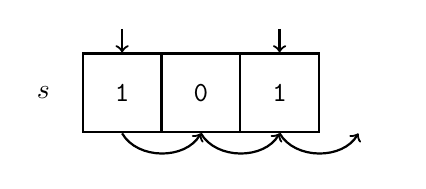
\begin{tikzpicture}[node distance=2cm, thick]
    % Nós para os números
    \node[draw = none] (s) at (0,0) {$s$};
    \node[draw, rectangle, minimum width=1cm, minimum height=1cm] (s1) at (1,0) {\tt 1};
    \node[draw, rectangle, minimum width=1cm, minimum height=1cm] (s2) at (2,0) {\tt 0};
    \node[draw, rectangle, minimum width=1cm, minimum height=1cm] (s3) at (3,0) {\tt 1};
    \node[draw = none, rectangle, minimum width=1cm, minimum height=1cm] (s4) at (4,0) {};

    % Setas pequenas em cima do primeiro e do último número
    \draw[->] ([yshift=0.3cm]s1.north) -- (s1.north);
    \draw[->] ([yshift=0.3cm]s3.north) -- (s3.north);
    
    % Setas abauladas embaixo
    \draw[->, out=-60, in=-120] (s1.south) to (s2.south);
    \draw[->, out=-60, in=-120] (s2.south) to (s3.south);
    \draw[->, out=-60, in=-120] (s3.south) to (s4.south);
  \end{tikzpicture}
\end{center}
  
O novo bit a ser inserido na primeira posição é: $1 \xor 1 = 0$

O primeiro bit produzido é {\tt 1} que é o bit que estava na última posição.

\begin{center}
  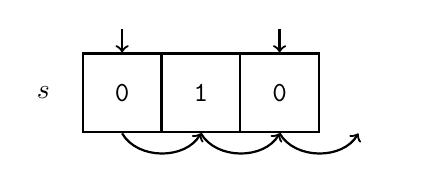
\begin{tikzpicture}[node distance=2cm, thick]
    % Nós para os números
    \node[draw = none] (s) at (0,0) {$s$};
    \node[draw, rectangle, minimum width=1cm, minimum height=1cm] (s1) at (1,0) {\tt 0};
    \node[draw, rectangle, minimum width=1cm, minimum height=1cm] (s2) at (2,0) {\tt 1};
    \node[draw, rectangle, minimum width=1cm, minimum height=1cm] (s3) at (3,0) {\tt 0};
    \node[draw = none, rectangle, minimum width=1cm, minimum height=1cm] (s4) at (4,0) {};

    % Setas pequenas em cima do primeiro e do último número
    \draw[->] ([yshift=0.3cm]s1.north) -- (s1.north);
    \draw[->] ([yshift=0.3cm]s3.north) -- (s3.north);
    
    % Setas abauladas embaixo
    \draw[->, out=-60, in=-120] (s1.south) to (s2.south);
    \draw[->, out=-60, in=-120] (s2.south) to (s3.south);
    \draw[->, out=-60, in=-120] (s3.south) to (s4.south);
  \end{tikzpicture}
\end{center}

O novo bit a ser inserido na primeira posição é: $0 \xor 0 = 0$

O segundo bit produzido é {\tt 0} que é o bit que estava na última posição.

\begin{center}
  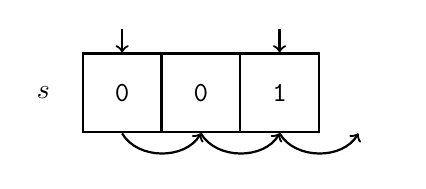
\begin{tikzpicture}[node distance=2cm, thick]
    % Nós para os números
    \node[draw = none] (s) at (0,0) {$s$};
    \node[draw, rectangle, minimum width=1cm, minimum height=1cm] (s1) at (1,0) {\tt 0};
    \node[draw, rectangle, minimum width=1cm, minimum height=1cm] (s2) at (2,0) {\tt 0};
    \node[draw, rectangle, minimum width=1cm, minimum height=1cm] (s3) at (3,0) {\tt 1};
    \node[draw = none, rectangle, minimum width=1cm, minimum height=1cm] (s4) at (4,0) {};

    % Setas pequenas em cima do primeiro e do último número
    \draw[->] ([yshift=0.3cm]s1.north) -- (s1.north);
    \draw[->] ([yshift=0.3cm]s3.north) -- (s3.north);
    
    % Setas abauladas embaixo
    \draw[->, out=-60, in=-120] (s1.south) to (s2.south);
    \draw[->, out=-60, in=-120] (s2.south) to (s3.south);
    \draw[->, out=-60, in=-120] (s3.south) to (s4.south);
  \end{tikzpicture}
\end{center}

O novo bit a ser inserido na primeira posição é: $0 \xor 1 = 1$

O terceiro bit produzido é {\tt 1} que é o bit que estava na última posição.

\begin{center}
  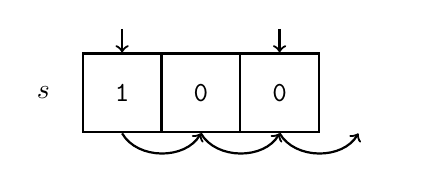
\begin{tikzpicture}[node distance=2cm, thick]
    % Nós para os números
    \node[draw = none] (s) at (0,0) {$s$};
    \node[draw, rectangle, minimum width=1cm, minimum height=1cm] (s1) at (1,0) {\tt 1};
    \node[draw, rectangle, minimum width=1cm, minimum height=1cm] (s2) at (2,0) {\tt 0};
    \node[draw, rectangle, minimum width=1cm, minimum height=1cm] (s3) at (3,0) {\tt 0};
    \node[draw = none, rectangle, minimum width=1cm, minimum height=1cm] (s4) at (4,0) {};

    % Setas pequenas em cima do primeiro e do último número
    \draw[->] ([yshift=0.3cm]s1.north) -- (s1.north);
    \draw[->] ([yshift=0.3cm]s3.north) -- (s3.north);
    
    % Setas abauladas embaixo
    \draw[->, out=-60, in=-120] (s1.south) to (s2.south);
    \draw[->, out=-60, in=-120] (s2.south) to (s3.south);
    \draw[->, out=-60, in=-120] (s3.south) to (s4.south);
  \end{tikzpicture}
\end{center}

O novo bit a ser inserido na primeira posição é: $1 \xor 0 = 1$

O quarto bit produzido é {\tt 0} que é o bit que estava na última posição.

Portanto, os primeiros bits da sequência gerada seriam: {\tt 1}, {\tt 0}, {\tt 1}, {\tt 0}.

\end{example}


Um RDRL com $n$ registradores é capaz de gerar no máximo $2^n - 1$ bits antes de começar a repetir sua sequência.
Isso ocorre porque o número de estados possíveis para um vetor de registradores com $n$ bits é $2^n$, e o estado em que todos os bits são 0 não é válido-- se ele ocorresse, o RDRL continuaria gerando apenas 0s indefinidamente.
Assim, depois de no máximo $2^n - 1$ passos, o RDRL retornará a um estado anterior, iniciando assim um ciclo.

O tamanho do ciclo de um RDRL refere-se ao número de bits gerados antes que a sequência comece a se repetir.
Em outras palavras, é o período da sequência pseudo-aleatória produzida pelo RDRL.
Um bom RDRL é aquele que tem um ciclo longo, idealmente próximo de $2^n - 1$, o que significa que ele pode gerar uma longa sequência de bits únicos antes de repetir.

Como discutido anteriormente, o comportamento de um RDRL é definido por um vetor de bits que determina o coeficiente de realimentação.
Dado um RDRL com $n$ registradores, certos vetores de feedback produzem ciclos ideais, enquanto outros não.
Os vetores que geram um ciclo ideal representam polinômios irredutíveis de grau $n$.
Um polinômio irredutível é aquele que não pode ser fatorado em polinômios de grau menor -- eles funcionam como números primos no universo dos polinômios\footnote{No Apêndice \ref{cha:corpos-finitos} apresentamos alguns exemplos.}.

Por exemplo, o polinômio $x^3 + x^2 + x + 1$ (representado pelo vetor binário $1111_2$) pode ser fatorado como $(x^2 + 1)(x + 1)$ no caso de coeficientes binários, que é o nosso contexto.
Por outro lado, o polinômio $x^3 + x + 1$ (representado pelo vetor binário \(1011_2\)) é irredutível.
Portanto, para um registrador de 4 bits, o vetor binário $1011_2$ gera um ciclo ideal de tamanho $2^4 - 1 = 15$, enquanto o vetor $1111_2$ não produz um ciclo ideal.
Contudo, não demonstraremos formalmente este resultado. 

A linearidade dos RDRLs é um problema, pois torna previsível antecipar os próximos bits gerados com base nos anteriores.
Essa previsibilidade compromete a segurança de sistemas de cifra de fluxo.

Na próxima seção, veremos como combinar múltiplos RDRLs de forma a quebrar essa linearidade, produzindo assim um GNP mais robusto e seguro, adequado para aplicações criptográficas.

%O segredo de um RDRL, ou sua ``chave'', é a semente $s_0 \dots s_{n-1}$.
%Lembre-se de que assumimos que o mecanismo (neste caso, os coeficientes de feedback) é sempre conhecido publicamente. Isso significa que qualquer segurança do sistema depende exclusivamente da semente inicial.

%Um ataque relativamente simples a um RDRL envolve a observação dos $n$ primeiros bits gerados, \(y_{n+1}, \dots, y_{2n}\), e a resolução de um sistema linear.
%A ideia é que, conhecendo os primeiros bits gerados, podemos inferir os coeficientes de feedback e, portanto, prever os próximos bits gerados pelo RDRL.

%Quando observamos os $n$ primeiros bits gerados pelo RDRL, podemos configurar um sistema de equações lineares para resolver os coeficientes de feedback.
%Considere os bits $y_1, y_2, \dots, y_{2n}$ gerados pelo RDRL.
%Podemos expressar cada bit como uma combinação linear dos bits anteriores, ponderada pelos coeficientes de feedback $c_0, c_1, \dots, c_{n-1}$:

%\begin{displaymath}
%  \begin{array}{rcl}
%    y_{n+1} & = & c_0y_1 \oplus c_1y_{n-1} \oplus \cdots \oplus c_{n-1} y_1 \\
%    y_{n+2} & = & c_0y_{n+1} \oplus c_1y_n \oplus \cdots \oplus c_{n-1} y_2 \\
%    & \vdots & \\
%    y_{2n} & = & c_0y_{2n-1} \oplus c_1y_{2n-2} \oplus \cdots \oplus c_{n-1} y_n \\
%  \end{array}
%\end{displaymath}

%É possível mostrar que essas equações são linearmente independentes e, portanto, elas determinam unicamente os coefientes.
%Uma vez determinados os valores $y_0 \dots y_n = s_0 \dots s_n$, podemos prever cada novo bit da sequência.
%Com isso torna-se simples a tarefa de construir um distinguidor para o gerador.

%\begin{example}
%  Vamos considerar que os coeficientes de feedback são $c_0 = 1$, $c_1 = 0$, $c_2 = 1$.

%  O adversário sabe esses valores porque isso é parte do mecanismo.

%  Imagine que observamos os três primeiros valores: $y_4 = 0$, $y_5 = 1$ e $y_6 = 0$.
%  Temos então que:

%  \begin{displaymath}
%    \begin{array}{rcl}
%      y_1 \oplus y_3 & = & 0 \\
%      y_2 \oplus y_4 & = & 1 \\
%      y_2 \oplus 0 & = & 1\\
%      y_2 & = & 1 \\
%    \end{array}
%  \end{displaymath}

%  \begin{displaymath}
%    \begin{array}{rcl}
%      y_3 \oplus y_5 & = & 0 \\
%      y_3 \oplus 1 & = & 0 \\
%      y_3 & = & 1 \\
%    \end{array}
%  \end{displaymath}

%  \begin{displaymath}
%    \begin{array}{rcl}
%      y_1 \oplus y_3 & = & 0 \\
%      y_1 \oplus 1 & = &  0\\
%      y_1 & = & 1 \\
%    \end{array}
%  \end{displaymath}

%  Portanto, a semente inicial é $y_1 = 1$, $y_2 = 1$ e $y_3 = 1$.

%  Usando os bits observados e os coeficientes de feedback conhecidos, fomos capazes de determinar a semente inicial do RDRL.
%  Isso demonstra como um adversário pode comprometer a segurança do RDRL ao observar um número suficiente de bits gerados.
%\end{example}

O RDRL não é considerado seguro para aplicações criptográficas porque a operação que gera novos bits é linear.
Essa linearidade permite que o RDRL seja previsível e, portanto, vulnerável a ataques.
Um adversário que observa um número suficiente de bits gerados pelo RDRL pode resolver um sistema de equações lineares para determinar a semente inicial e, consequentemente, prever todos os bits subsequentes.

Embora os RDRLs não sejam seguros, muitos Geradores de Números Pseudo-Aleatórios (GNPs) usados na prática são versões modificadas deste esquema geral.
A segurança dos GNPs modernos geralmente depende da introdução de não-linearidades no processo de geração de bits.
Em vez de usar exclusivamente operações lineares como a XOR, os GNPs seguros utilizam funções não lineares.
Essas funções podem incluir operações aritméticas complexas, substituições de bits baseadas em tabelas (substituições S-box) ou outras transformações matemáticas que dificultam a previsão dos bits gerados.

\subsection{Trivium}
\label{sec:trivium}

Em 2008, um concurso científico focado na produção de cifras de fluxo seguras foi realizado com o objetivo de identificar algoritmos que fossem tanto seguros quanto eficientes.
Este concurso, conhecido como projeto eSTREAM, reuniu diversas propostas de algoritmos de criptografia de fluxo, cada um competindo para se destacar como uma solução viável para a criptografia moderna.

Entre os algoritmos selecionados pelo projeto eSTREAM, o {\em Trivium} \cite{DeCanniere06} se destacou como uma alternativa segura e eficiente.
O Trivium foi desenvolvido por Christophe De Canniere e Bart Preneel em 2006.
Este algoritmo é projetado para ser simples e leve, mas ao mesmo tempo, capaz de oferecer alto grau de segurança.

O Trivium recebe dois valores como entrada, ambos com 80 bits:
\begin{enumerate}
\item {\em Semente (Key)}: Uma sequência de 80 bits que serve como chave secreta do algoritmo.
\item {\em Vetor Inicial (VI)}: Outra sequência de 80 bits, que é usada para garantir a unicidade da cifra gerada para diferentes mensagens, mesmo quando a mesma chave é utilizada.
\end{enumerate}

O estado interno do Trivium é representado por um vetor de 288 bits.
Esse estado é atualizado iterativamente para gerar a sequência de saída pseudo-aleatória.
A atualização do estado é projetada de tal forma que o ciclo do Trivium tem um tamanho de $2^{64}$ bits, ou seja, o Trivium pode gerar uma sequência de até $2^{64}$ bits antes de começar a repetir.

Até o momento, o Trivium tem resistido a uma ampla gama de ataques criptoanalíticos, o que reforça sua reputação como um algoritmo seguro.
Além disso, ele é eficiente em termos de uso de recursos computacionais, tornando-o adequado para aplicações com restrições de hardware, como dispositivos embarcados.

\subsection*{Estrutura e Funcionamento do Trivium}

O Trivium possui três registradores denominados A, B e C, com tamanhos de 93, 84 e 111 bits, respectivamente, totalizando 288 bits.

A inicializaćão dos registradores é feita da seguinte forma:

\begin{enumerate}
\item {\em Chave (Key)}:
  \begin{itemize}
  \item A chave de 80 bits é inserida nas primeiras posições do registrador A.
  \item As demais posições do registrador A são preenchidas com zeros.
  \end{itemize}
  
\item {\em Vetor Inicial ($VI$)}:
  \begin{itemize}
  \item O vetor inicial de 80 bits é inserido nas últimas posições do registrador B.
  \item As demais posições do registrador B são preenchidas com zeros.
  \end{itemize}
    
\item Todas as posições do registrador C são preenchidas com zeros, exceto as últimas três posições, que são preenchidas com uns.    
\end{enumerate}

Antes de começar a produzir o fluxo de bits, o Trivium passa por uma {\em fase de aquecimento}.
Durante esta fase, o algoritmo roda $4 \times 288 = 1152$ ciclos para misturar completamente o estado interno.
Esta fase de aquecimento ajuda a assegurar que o estado inicial não revele diretamente a chave ou o vetor inicial.

Os passos seguintes do Trivium são:
\begin{enumerate}
    \item {\em Cálculo do Bit de Saída}:
    \begin{itemize}
        \item Cada registrador calcula o AND entre o penúltimo e o antepenúltimo bit.
        \item O resultado é então combinado usando XOR com o último bit e com um bit de uma posição fixa chamada de {\em feedforward bit}.
        \item Este cálculo gera o \textit{bit de saída}.
    \end{itemize}
    
    \item {\em Envio do Bit de Saída}:
    \begin{itemize}
        \item O bit de saída de cada registrador é enviado para o registrador adjacente:
        \begin{itemize}
            \item Registrador A envia seu bit de saída para o registrador B.
            \item Registrador B envia seu bit de saída para o registrador C.
            \item Registrador C envia seu bit de saída para o registrador A.
        \end{itemize}
    \end{itemize}
    
    \item {\em Deslocamento dos Bits}:
    \begin{itemize}
        \item Cada registrador desloca seus bits uma posição para a direita, semelhante ao RDRL.
    \end{itemize}
    
    \item {\em Inserção do Novo Bit}:
    \begin{itemize}
        \item Cada registrador aplica XOR entre o bit recebido e um bit de uma posição fixa chamada de {\em feedbackward bit}.
        \item O resultado é inserido na primeira posição do registrador.
    \end{itemize}
    
    \item {\em Geração do Bit de Fluxo}:
    \begin{itemize}
        \item O XOR dos três bits de saída dos registradores A, B e C é calculado.
        \item Este resultado final é o bit do fluxo gerado pelo Trivium.
    \end{itemize}
\end{enumerate}

\begin{tikzpicture}[scale=0.8]
    % Registrador 1 (93 bits)
    \draw (0,0) rectangle (9.3,1) node[pos=.5] {A (93 bits)};
    
    % Espaço entre os registradores
    \draw (0,-3) rectangle (8.4,-2) node[pos=.5] {B (84 bits)};
    
    % Registrador 3 (111 bits)
    \draw (0,-6) rectangle (11.1,-5) node[pos=.5] {C (111 bits)};

    % Saída do bit 69 do Registrador 1
    \node at (6.9, 0.5) (bit69) {};
    \node at (-1, 0.5) (xorBeforeA) {\Large $\xor$}; % Símbolo de XOR
    \node at (0, 0.5) (inicioR1) {};

    % Desenha a seta do bit 69 subindo, voltando e descendo até o XOR com curvas arredondadas
  %  \draw[->] (6.9, 1) to[out=90, in=0] (3.5, 1.5) to[out=180, in=90] (-1, 1.5) -- (xorBeforeA);

    
    % Desenha a seta do bit 69 subindo, voltando e descendo até o XOR
    \draw[->] (6.9, 1) to[out=90, in=0] (6, 1.5) -- (0, 1.5) to[out=180, in=90] (xorBeforeA);

    % Desenha a seta do XOR para o início do registrador 1
    \draw[->] (xorBeforeA) -- (inicioR1);

    \node at (7.8, -2.5) (bit78) {};
    \node at (-1, -2.5) (xorBeforeB) {\Large $\xor$}; % Símbolo de XOR
    \node at (0, -2.5) (inicioR2) {};

    %    \draw[->] (7.8, -2) -- (7.8, -1.5) -- (-1, -1.5) -- (xorBeforeB);
    \draw[->] (7.8, -2) to[out=90, in=0] (7, -1.5) -- (0, -1.5) to[out=180, in=90] (xorBeforeB);

    \draw[->] (xorBeforeB) -- (inicioR2);

    \node at (8.7, -5.5) (bit87) {};
    \node at (-1, -5.5) (xorBeforeC) {\Large $\xor$}; % Símbolo de XOR
    \node at (0, -5.5) (inicioR3) {};

%    \draw[->] (7.8, -5) -- (7.8, -4.5) -- (-1, -4.5) -- (xorBeforeC);
    \draw[->] (7.8, -5) to[out=90, in=0] (7, -4.5) -- (0, -4.5) to[out=180, in=90] (xorBeforeC);

    \draw[->] (xorBeforeC) -- (inicioR3);

    % Adicionar porta lógica AND rotacionada abaixo das posições 91 e 92
    \node at (9.1, 1) (bit91) {};
    \node at (9.2, 1) (bit92) {};
    \node[and gate US, draw, logic gate inputs=nn, rotate=-90, xscale=0.6] (andgate) at (9.15, -0.5) {}; % Porta lógica AND rotacionada
    
    % Conectar os bits 91 e 92 à porta AND rotacionada
    \draw[->] (9.1, 0) -- (andgate.input 2);
    \draw[->] (9.2, 0) -- (andgate.input 1);

    % Adicionar um novo XOR após o Registrador A
    \node at (10.5, 0.5) (xorAfterA) {\Large $\xor$}; 
    
    % Desenhar uma seta do registrador A para o XOR novo
    \draw[->] (9.3, 0.5) -- (xorAfterA);
    
    % Desenhar uma seta da porta AND para o XOR novo
%    \draw[->] (andgate.output) -- (9.15, -1) -- (10.5, -1) -- (xorAfterA);
    \draw[->] (andgate.output) to[out=270, in=180] (9.5, -1) -- (10.2, -1) to[out=0, in=270] (xorAfterA);

    

    % Adicionar porta lógica AND rotacionada abaixo das posições 82 e 83
    \node at (8.2, -2) (bit82) {};
    \node at (8.3, -2) (bit83) {};
    \node[and gate US, draw, logic gate inputs=nn, rotate=-90, xscale=0.6] (andgate2) at (8.25, -3.5) {}; % Porta lógica AND rotacionada
    
    % Conectar os bits 82 e 83 à porta AND rotacionada
    \draw[->] (8.2, -3) -- (andgate2.input 2);
    \draw[->] (8.3, -3) -- (andgate2.input 1);

    % Adicionar um novo XOR após o Registrador B
    \node at (9.5, -2.5) (xorAfterB) {\Large $\xor$}; 
    
    % Desenhar uma seta do registrador B para o XOR novo
    \draw[->] (8.4, -2.5) -- (xorAfterB);
    
    % Desenhar uma seta da porta AND para o XOR novo
    %\draw[->] (andgate2.output) -- (8.25, -4) -- (9.5, -4) -- (xorAfterB);
    \draw[->] (andgate2.output) to[out=270, in=180] (8.5, -4) -- (9.2, -4) to[out=0, in=270] (xorAfterB);
    
    % Adicionar porta lógica AND rotacionada abaixo das posições 109 e 110
    \node at (10.9, -5) (bit109) {};
    \node at (11, -5) (bit110) {};
    \node[and gate US, draw, logic gate inputs=nn, rotate=-90, xscale=0.6] (andgate3) at (10.95, -6.5) {}; % Porta lógica AND rotacionada
    
    % Conectar os bits 82 e 83 à porta AND rotacionada
    \draw[->] (10.9, -6) -- (andgate3.input 2);
    \draw[->] (11, -6) -- (andgate3.input 1);

    % Adicionar um novo XOR após o Registrador A
    \node at (12, -5.5) (xorAfterC) {\Large $\xor$}; 
    
    % Desenhar uma seta do registrador C para o XOR novo
    \draw[->] (11.1, -5.5) -- (xorAfterC);
    
    % Desenhar uma seta da porta AND para o XOR novo
 %   \draw[->] (andgate3.output) -- (10.95, -7) -- (12, -7) -- (xorAfterC);
    \draw[->] (andgate3.output) to[out=270, in=180] (11.2, -7) -- (11.7, -7) to[out=0, in=270] (xorAfterC);
    
    % Desenha a seta do bit 66 subindo, indo e descendo até o XORAfterA
%    \draw[->] (6.6, 1) -- (6.6, 1.7) -- (10.5, 1.7) -- (xorAfterA);
    \draw[->] (6.6, 1) to[out=90, in=180] (7.3, 1.7) -- (9.8, 1.7)  to[out=0, in=90] (xorAfterA);


    % Desenha a seta do bit 69 subindo, indo e descendo até o XORAfterB
%    \draw[->] (6.9, -2) -- (6.9, -1.3) -- (9.5, -1.3) -- (xorAfterB);
    \draw[->] (6.9, -2) to[out=90, in=180] (7.6, -1.3) -- (8.8, -1.3)  to[out=0, in=90] (xorAfterB);
    
    % Desenha a seta do bit 69 subindo, indo e descendo até o XORAfterB
%    \draw[->] (6.6, -5) -- (6.6, -4.3) -- (12, -4.3) -- (xorAfterC);
    \draw[->] (6.6, -5) to[out=90, in=180] (7.3, -4.3) -- (11.3, -4.3)  to[out=0, in=90] (xorAfterC);
    
    % Adicionar um novo XOR foward
    \node at (13, -2.5) (xorFoward) {\Large $\xor$}; 

    % Desenha a seta do XorAfterA até o XorFoward
%    \draw[->] (xorAfterA) -- (13, 0.5) -- (xorFoward);
    \draw[->] (xorAfterA) to[out=0, in=180] (12.2, 0.5) to[out=0, in=90] (xorFoward);


    % Desenha a seta do XorAfterB até o XorFoward
    \draw[->] (xorAfterB) -- (xorFoward);

    % Desenha a seta do XorAfterC até o XorFoward
    %\draw[->] (xorAfterC) -- (13, -5.5) -- (xorFoward);
    \draw[->] (xorAfterC) to[out=0, in=180] (12.3, -5.5) to[out=0, in=270] (xorFoward);

    % Desenha a seta do XorFoward pra fora
    \draw[->] (xorFoward) -- (14, -2.5);

    % Desenha a seta do XorAfterA pra xorBeforeB
   % \draw[->] (11, 0.5) -- (11, -1.1) -- (-1.7, -1.1) -- (-1.7, -2.5) -- (xorBeforeB);
    \draw[->] (11.2, 0.5)
          to[out=270, in=0] (10.7, -1.1) 
          to[out=180, in=0] (-1.3, -1.1) 
          to[out=180, in=180] (-1.5, -2.5) -- (xorBeforeB);


    % Desenha a seta do XorAfterB pra xorBeforeC
    %\draw[->] (10, -2.5) -- (10, -4.1) -- (-1.7, -4.1) -- (-1.7, -5.5) -- (xorBeforeC);
    \draw[->] (10.2, -2.5)
          to[out=270, in=0] (9.7, -4.1) 
          to[out=180, in=0] (-1.3, -4.1) 
          to[out=180, in=180] (-1.5, -5.5) -- (xorBeforeC);

    % Desenha a seta do XorAfterC pra xorBeforeA
          %\draw[->] (12.5, -5.5) -- (12.5, -7.1) -- (-2, -7.1) -- (-2, 0.5) -- (xorBeforeA);
    % Desenha a seta do XorAfterC para xorBeforeA com curvas arredondadas
    \draw[->] (12.5, -5.5) to[out=0, in=0] (12.8, -7.1) 
          to[out=180, in=0] (-1, -7.1) 
          to[out=180, in=270] (-2.8, -3.5) 
          to[out=90, in=180] (-1.5, 0.5) -- (xorBeforeA);

\end{tikzpicture}

Resumindo, o Trivium é um algoritmo de cifra de fluxo que utiliza três registradores interligados para gerar uma sequência pseudoaleatória de bits.
Em cada passo, os registradores realizam operações lógicas e de deslocamento, trocando bits de saída entre si e inserindo novos bits com base em cálculos de feedback.
A combinação dos bits de saída dos três registradores gera o fluxo de bits que é usado para criptografar ou descriptografar mensagens.

A Tabela \ref{tab:trivium} resume as especificações do Trivium, a posição do feedack-bit e do feed-foward bit de cada um dos três registradores.

\begin{table}[h!]
  \label{tab:trivium}
\centering
\begin{tabular}{|c|c|c|c|}
\hline
\textbf{Registrador} & \textbf{Feedback Bit} & \textbf{Feedforward Bit} & \textbf{Tamanho} \\
\hline
A & 69 & 66 & 93 \\
\hline
B & 78 & 69 & 84 \\
\hline
C & 87 & 66 & 111 \\
\hline
\end{tabular}
\caption{Especificações do Trivium}
\end{table}

A escolha de um bom gerador de números pseudo-aleatórios (GNP) é crucial para garantir a segurança de uma cifra de fluxo.
Utilizar geradores inadequados pode comprometer seriamente a integridade do sistema criptográfico.
Um erro comum é utilizar funções padrão de bibliotecas de programação, como a função \texttt{rand} da biblioteca padrão da linguagem \texttt{C}.
Embora essas funções sejam adequadas para simulações e outras aplicações não críticas, elas não oferecem o nível de segurança necessário para aplicações criptográficas.

Para garantir a segurança de sistemas criptográficos, é essencial utilizar GNPs que foram rigorosamente avaliados e validados pela comunidade criptográfica.
A orientação geral é utilizar geradores selecionados pelo projeto eSTREAM, que foram submetidos a testes extensivos e demonstraram ser seguros contra uma variedade de ataques criptoanalíticos.
Dois exemplos notáveis de geradores aprovados pelo projeto eSTREAM são o Trivium, que foi detalhado nesta seção, e o SALSA20.


\section{Exercicios}
\label{sec:exercicios}

\begin{exercicio}
  O que precisamos assumir para que um sistema de criptografia baseado em cifra de fluxo seja seguro?

  Em que sentido podemos considerá-lo seguro?
\end{exercicio}

\begin{exercicio}
Mostre que o gerador $G$ com fator de expansão $l(n) = n + 1$ que recebe $s \in \{0,1\}^n$ e devolve $s$ concatenado com $\bigoplus_{i=0}^ns_i$ não é um GNP.  
\end{exercicio}

\begin{exercicio}
  Construa um dintinguidor eficiente $D$ para o RDRL simples.
\end{exercicio}

\begin{exercicio}
  Por que em uma cifra de fluxo não podemos criptografar duas mensagens distintas com a mesma chave?
\end{exercicio}

\begin{exercicio}
 Sejam $y_0, y_1, y_2 \dots$ os bits gerados pelo algoritmo RC4.
É possível mostrar que para uma distribuição uniforme de sementes e vetores iniciais, a probabilidade dos bits $y_9, \dots, y_{16}$ serem todos iguais a $0$ é $\frac{2}{256}$.
Mostre como construir um algoritmo eficiente $D$ capaz de distinguir as sequências de bits produzidas pelo RC4 de uma sequência realmente aleatória.
\end{exercicio}

\begin{exercicio}
  Considere a seguinte implementação de uma cifra de fluxo:
\begin{enumerate}
\item Utilizamos o número de segundos desde primeiro de janeiro de 1970 até o momento atual para gerar uma semente $s$ que armazenamos em um local seguro.
\item Utilizamos, então, a implementação {\tt rand} da biblioteca padrão do {\tt C} para gerar uma sequência de $n$ bits $G(s)$.
\item Produzimos a cifra $c = G(s) \xor m$ supondo que $|m| = n$.
\item Para descriptografar recuperamos $s$, aplicamos $G(s) \xor c$.
\end{enumerate}

  Descreva duas vulnerabilidades deste protocolo.
\end{exercicio}


